\section{Analysis}
\label{sec:analysis}



% \begin{figure}[t!]
% \centering

% \subfloat{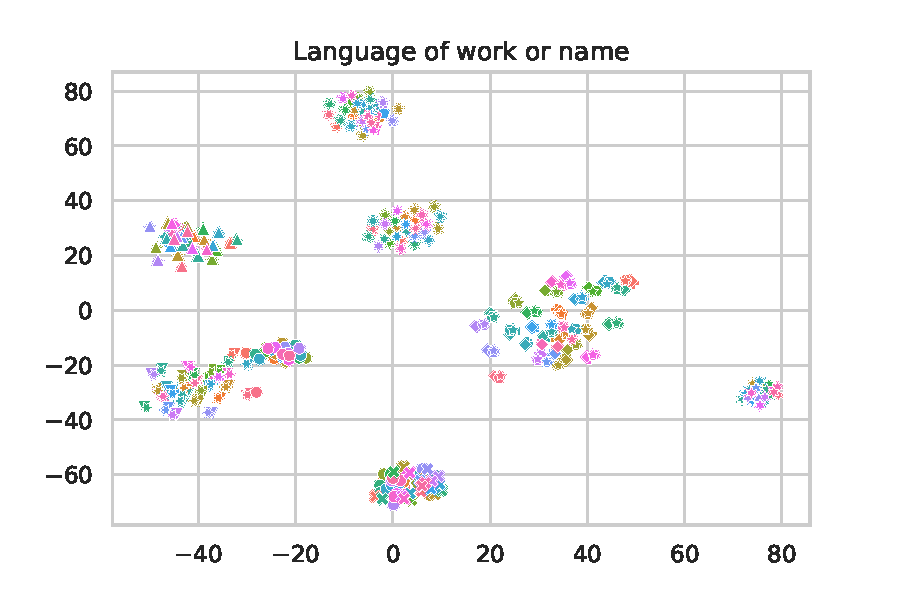
\includegraphics[width=1.\columnwidth]{figures/P407_emb.pdf}}\\
% %   \hfill
% \subfloat{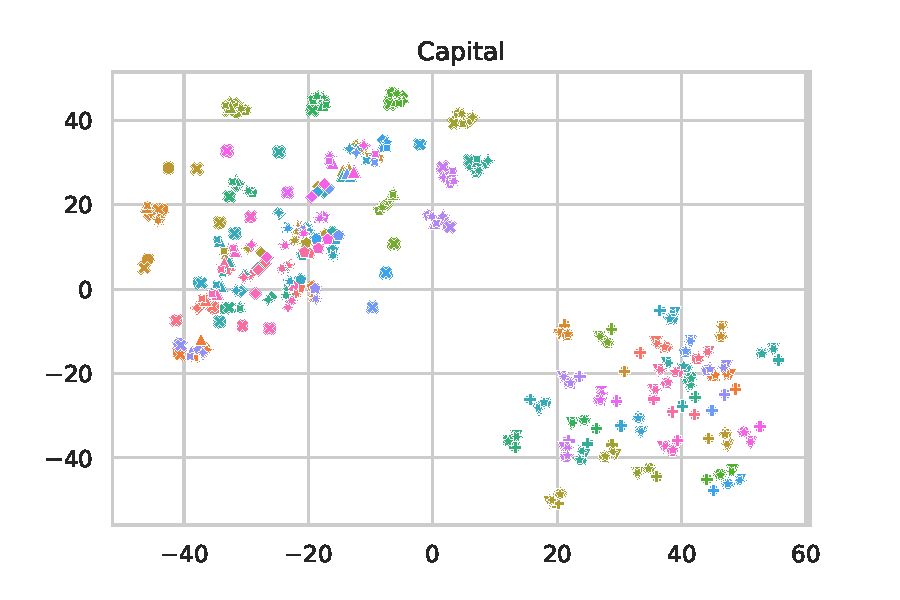
\includegraphics[width=1.\columnwidth]{figures/P36_emb.pdf}}
% % \\


% \caption{t-SNE plots for encoded patterns from the ``Language of work or name'' and ``Capital'' relations. Points of the same color represent the same subject, Points of the same shape represent the same pattern. A consistent representation should cluster based on subjects (colors) rather than patterns (shapes).}
% \label{fig:tsne-emb}

% \end{figure}

\begin{table*}[t]
% \small
    \centering
\resizebox{1\textwidth}{!}{%
\begin{tabular}{llllllll}
\toprule
Subject & Object & Pattern \#1 & Pattern \#2 & Pattern \#3 & Pred \#1 & Pred \#2 & Pred \#3 \\
\midrule

% Adam Kendon & London & [X] was born in [Y]. & [X] is originally from [Y]. & The country of origin of [X] is [Y]. & \hltrue{London} & \hltrue{London} & \hlfalseo{Ireland} \\
Adriaan Pauw & Amsterdam & [X] was born in [Y]. & [X] is native to [Y]. & [X] is a [Y]-born person. & \hltrue{Amsterdam} & \hlfalseo{Madagascar} & \hlfalset{Luxembourg} \\
Nissan Livina Geniss & Nissan & [X] is produced by [Y]. & [X] is created by [Y]. & [X], created by [Y]. & \hltrue{Nissan} & \hlfalseo{Renault} & \hlfalseo{Renault} \\
Arab League & Asia & [X] belongs to the continent of [Y]. & [X] is located in [Y]. &  [X] is a part of the continent of [Y]. & \hltrue{Asia} & \hlfalseo{Europe} & \hlfalset{Africa} \\ 
% Albania & Serbia & [X] shares border with [Y]. & [Y] borders with [X]. & [Y] shares the border with [X] & \hlfalseo{Greece} & \hlfalset{Turkey} & \hlfalsetr{Kosovo} \\
iCloud & Apple & [X] is developed by [Y]. & [X], created by [Y]. & [X] was created by [Y] & \hlfalseo{Microsoft} & \hlfalset{Google} & \hlfalsetr{Sony} \\
\midrule

Yahoo! Messenger & Yahoo & [X], a product created by [Y] & [X], a product developed by [Y] & [Y], that developed [X] & \hlfalseo{Microsoft} & \hlfalseo{Microsoft} & \hlfalseo{Microsoft} \\
Wales & Cardiff & The capital of [X] is [Y] . & [X]'s capital, [Y]. & [X]'s capital city, [Y]. & \hltrue{Cardiff} & \hltrue{Cardiff} & \hltrue{Cardiff} \\

\bottomrule
\end{tabular}


}
    \caption{Predictions of BERT-large-cased. Presenting the
      subjects and objects taken from T-REx \cite{trex}, as
      well as three different patterns from our resource and
      their predictions. The predictions are colored in blue
      if the model predicted correctly (out of the candidate
      list), and in red otherwise. If there is more than a
      single erroneous prediction, it is colored by a different red.}
    \label{tab:predictions}
\end{table*}


\subsection{Qualitative Analysis}
In order to better understand the factors affecting consistent predictions, we inspect multiple relations and their predictions. These patterns and their associated predictions are summarized in Table \ref{tab:predictions}.
We observe a range of phenomena. The predictions in the first row are consistent and correct for two patterns, but not to the third. However, the third pattern prediction is related in the sense that Ireland is close to London.
The last two rows in the first part show patterns that predict three different answers for the different paraphrases. Note that the first make predictions that are factually correct, but simply do not correspond to the gold object in t-REX (Greece and Kosovo), since this is an M-N relation. The second produces three different predictions which are all factually incorrect. Note that even when more than a single answer is correct, we still argue that the model should make consistent predictions.
Finally, the very last two rows demonstrate consistent predictions, which the first are factually incorrect (surprisingly due to the fact the object is a substring of the subject), and the second is consistent and factual.





\subsection{Representation Analysis}


To provide additional insights on the way models operate on the patterns with the masked tokens they need to predict, we inspect their representations after encoding the cloze-style patterns.

Encouraged from previous work that found that words with the same syntactic structure clusters together \cite{chi-etal-2020-finding,ravfogel-etal-2020-unsupervised} we perform a similar experiment to test if this behavior also occurs for knowledge.
We encode the patterns, after filling the placeholders with subjects and masked tokens and inspect the representation of the last layer in the masked token.
When plotting the results using t-SNE \cite{tsne} we mainly observe clustering based on the patterns \nk{If w say this, I would add a plot where this holds} \ye{no place}, which suggests that the knowledge, therefore the encoding of the entity's knowledge, is not the main component of the representations.
We also cluster these representations\footnote {Using the KMeans algorithm} using two number clusters \sr{sentence is not clear}: the number of patterns and the number of objects, and then measure the purity of these clusters, using V-measure. Generally, we observe that these clusters are clustered based on the patterns, rather than the objects.
Finally, we compute the correlation between the distance of two representations, and if their answers are consistent with each other. However, the correlation between these variables is very low (@@), therefore it does not explain alone the models' behavior.
These findings are interesting since it means that (1) these representations are not knowledge-focused, i.e. Their main component is not to encode knowledge, and (2) the entire representation does not explain the behavior of the model. This finding is consistent with previous work that observed similar trends for linguistic tasks \cite{amnesic_probing}.
We believe that the explanation of these findings is that the relevant information for the word prediction, lies in a subspace of the original representation, and thus much of the encoded information is in practice not relevant for the prediction. \sr{I don't understand this explanation. I'd write something like ``We hypothesize that this disparity between representation and behavior may be explained by a situation where distances between representations largely do not reflect the distance between predictions, but rather reflect other, behaviorally-irrelevant factors of each sentence"}.


% We encode the patterns, populated with 50 random subjects along with the masked token, and inspect the final layer in the masked token index for all the paraphrases of multiple relations.
% Then, we use t-SNE \cite{tsne} and present the results in Figure \ref{fig:tsne-emb} in the appendix.
% Each point represents a specific tuple, and are colored by the subjects, and the shape stands for the pattern.
% A good representation would cluster the vectors together based on the subject, as then the predictions would more likely to be consistent. However, clusters based on patterns would suggest a worse encoding, since the subjects, which are of great importance in these paraphrases, are less taken into account in the representation.

% We display the t-SNE figures for two relations, \textit{Language  of work or name} and \textit{Capital} in Figure \ref{fig:tsne-emb}.
% It is clear that the first figure clusters mainly on the patterns, whereas the second figure clusters mainly on the subjects. These results are also consistent with the performance of these relations: @@\% and @@\%, which suggests a better representation for the latter.
% Additionally, we also perform clustering for the representations,\footnote{Using the KMeans algorithm.} once with the number of subjects and once with the number patterns, given as an oracle, hoping to fit the subjects or patterns clusters. Then, we calculate the v-measure metric for measuring the purity of each cluster.
% A higher score on the subject-based would suggest a representation that better fits the purpose of a KB.
% The v-measure results for these patterns are presented in Table \ref{tab:vmeasure-small}.
% As expected, the pattern-based clustering is better for the \textit{language of work or name} relation is higher than the subject-based, and vice versa for the \textit{capital} relation.
% The full clustering measures for all relations are reported in the Appendix.
% \ar{Can we report correlation with performance for all relations here? Or say that in general we observe this trend?}
% \begin{table}[t]
% \small
    \centering
% \resizebox{1\textwidth}{!}{%
\begin{tabular}{lrr}
\toprule
                                          Pattern &  pattern &  subject \\
\midrule
     language of work or name &            0.72 &            0.24 \\
                      capital &            0.41 &            0.62 \\
\bottomrule
\end{tabular}

% }
    \caption{V-measure clustering performance for the two relations. Reporting the results for clustering based on the pattern, and based on the subjects.}
    \label{tab:vmeasure-small}
\end{table}


